\begin{figure}[!h]
  \vskip -0.25cm
  \begin{center}
    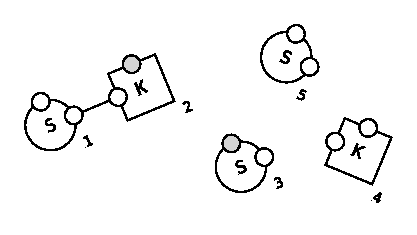
\includegraphics[scale=0.9]{figures/mixture.pdf}
  \end{center}
  \vskip -0.5cm
  \caption{An example of a reaction mixture. Instead of labelling
    sites with their names, we here identify them by their position on
    agents (phosphorylation sites are always shown on top). The
    relative position of agents in the figure is insignificant.
    Phosphorylated sites are shown in gray.  Number labels correspond
    to global agent identifiers. }
  \label{fig:mixture}
\end{figure}
